\subsection{Numerical prediction (low propagule, low synchrony, weak
omnivory)}\label{numerical-prediction-low-propagule-low-synchrony-weak-omnivory}

\begin{figure}
\centering
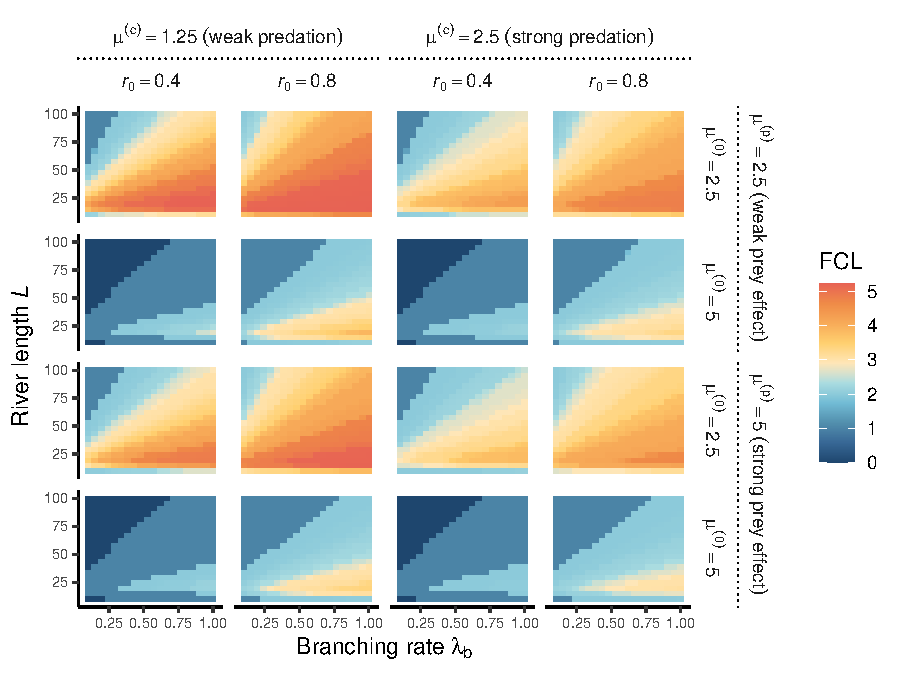
\includegraphics{../data_fmt/fig_rho025_g75_theta025.pdf}
\caption{Heatmap of FCL as a function of ecosystem size (river length,
\(L\)) and complexity (branching rate, \(\lambda_b\)), with rows and
columns displaying different combinations of resource supply (\(r_0\)),
disturbance regime (\(\mu^{(0)}\)), predation effect (\(\mu^{(c)}\)),
and prey effect (\(\mu^{(p)}\)). Each cell represents the average FCL of
five food webs. Additional parameter values are: number of gross
propagules \(g_0=75\), synchrony probability \(\rho=0.25\), omnivory
\(\theta=0.25\), habitat density \(h=2.5\), dispersal capability
\(\delta_0=0.5\), and scaling exponent \(\psi_1=\psi_2=0.5\).}
\end{figure}

\newpage

\subsection{Numerical prediction (high propagule, low synchrony, weak
omnivory)}\label{numerical-prediction-high-propagule-low-synchrony-weak-omnivory}

\begin{figure}
\centering
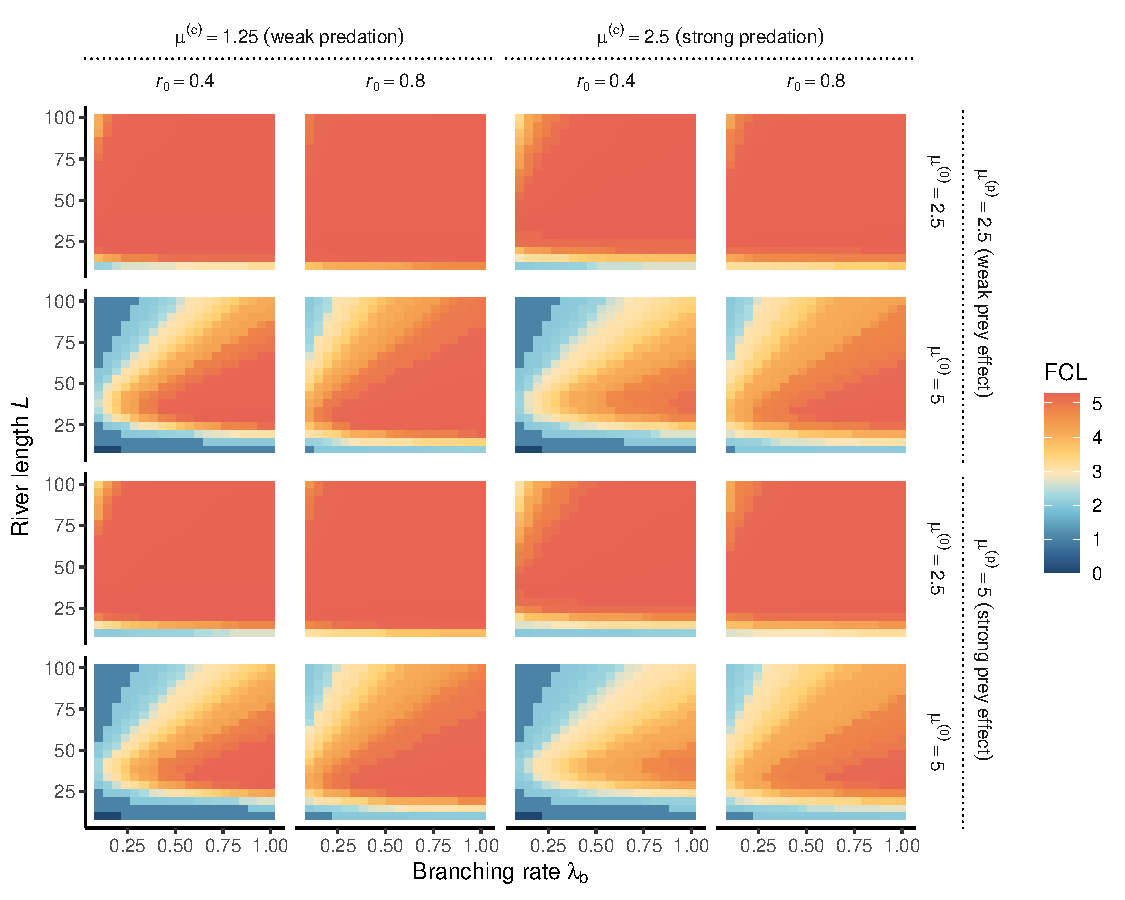
\includegraphics{../data_fmt/fig_rho025_g150_theta025.pdf}
\caption{Heatmap of FCL as a function of ecosystem size (river length,
\(L\)) and complexity (branching rate, \(\lambda_b\)), with rows and
columns displaying different combinations of resource supply (\(r_0\)),
disturbance regime (\(\mu^{(0)}\)), predation effect (\(\mu^{(c)}\)),
and prey effect (\(\mu^{(p)}\)). Each cell represents the average FCL of
five food webs. Additional parameter values are: number of gross
propagules \(g_0=150\), synchrony probability \(\rho=0.25\), omnivory
\(\theta=0.25\), habitat density \(h=2.5\), dispersal capability
\(\delta_0=0.5\), and scaling exponent \(\psi_1=\psi_2=0.5\).}
\end{figure}

\newpage

\subsection{Numerical prediction (low propagule, high synchrony, weak
omnivory)}\label{numerical-prediction-low-propagule-high-synchrony-weak-omnivory}

\begin{figure}
\centering
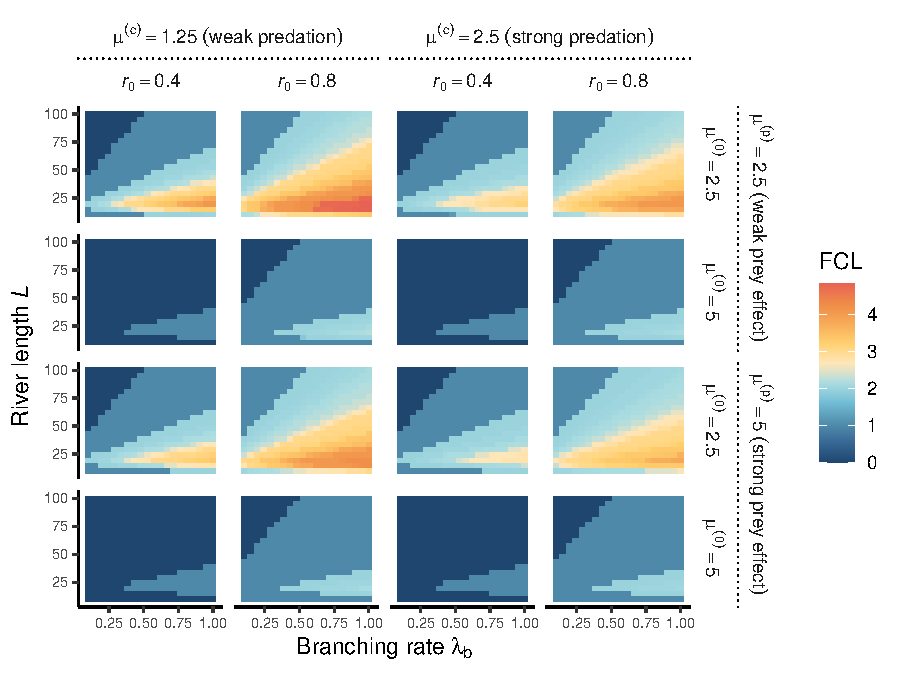
\includegraphics{../data_fmt/fig_rho05_g75_theta025.pdf}
\caption{Heatmap of FCL as a function of ecosystem size (river length,
\(L\)) and complexity (branching rate, \(\lambda_b\)), with rows and
columns displaying different combinations of resource supply (\(r_0\)),
disturbance regime (\(\mu^{(0)}\)), predation effect (\(\mu^{(c)}\)),
and prey effect (\(\mu^{(p)}\)). Each cell represents the average FCL of
five food webs. Additional parameter values are: number of gross
propagules \(g_0=75\), synchrony probability \(\rho=0.5\), omnivory
\(\theta=0.25\), habitat density \(h=2.5\), dispersal capability
\(\delta_0=0.5\), and scaling exponent \(\psi_1=\psi_2=0.5\).}
\end{figure}

\newpage

\subsection{Numerical prediction (high propagule, high synchrony, weak
omnivory)}\label{numerical-prediction-high-propagule-high-synchrony-weak-omnivory}

\begin{figure}
\centering
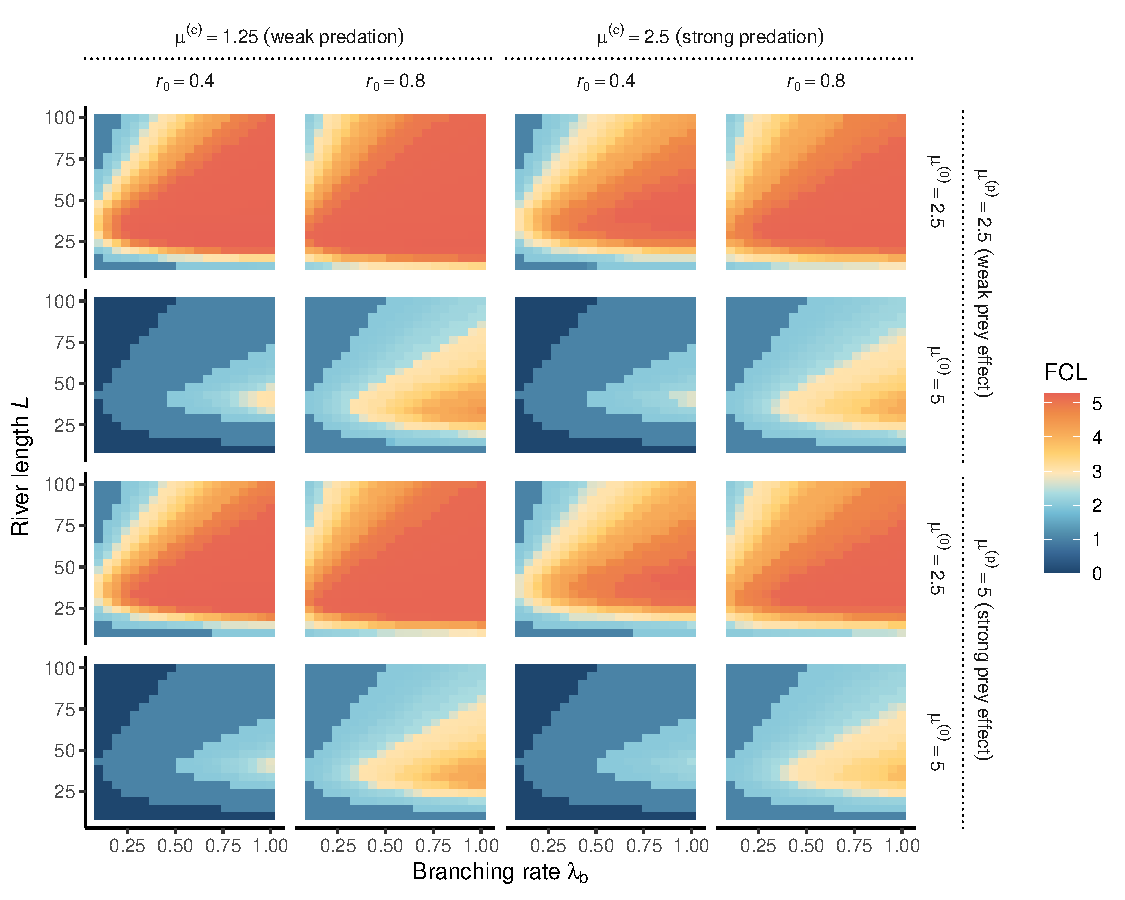
\includegraphics{../data_fmt/fig_rho05_g150_theta025.pdf}
\caption{Heatmap of FCL as a function of ecosystem size (river length,
\(L\)) and complexity (branching rate, \(\lambda_b\)), with rows and
columns displaying different combinations of resource supply (\(r_0\)),
disturbance regime (\(\mu^{(0)}\)), predation effect (\(\mu^{(c)}\)),
and prey effect (\(\mu^{(p)}\)). Each cell represents the average FCL of
five food webs. Additional parameter values are: number of gross
propagules \(g_0=150\), synchrony probability \(\rho=0.5\), omnivory
\(\theta=0.25\), habitat density \(h=2.5\), dispersal capability
\(\delta_0=0.5\), and scaling exponent \(\psi_1=\psi_2=0.5\).}
\end{figure}

\newpage

\subsection{Numerical prediction (low propagule, low synchrony, strong
omnivory)}\label{numerical-prediction-low-propagule-low-synchrony-strong-omnivory}

\begin{figure}
\centering
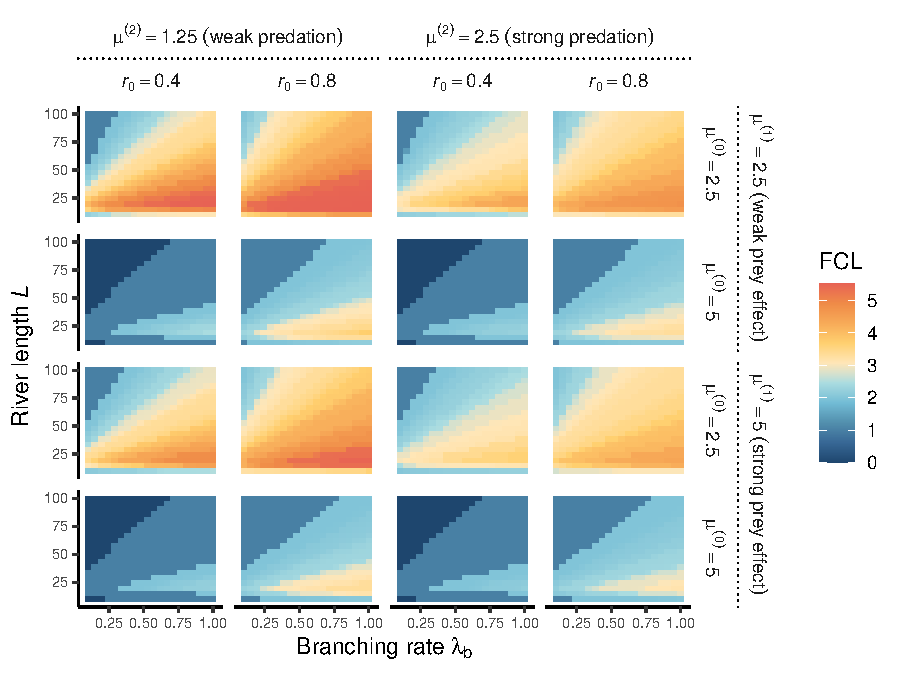
\includegraphics{../data_fmt/fig_rho025_g75_theta05.pdf}
\caption{Heatmap of FCL as a function of ecosystem size (river length,
\(L\)) and complexity (branching rate, \(\lambda_b\)), with rows and
columns displaying different combinations of resource supply (\(r_0\)),
disturbance regime (\(\mu^{(0)}\)), predation effect (\(\mu^{(c)}\)),
and prey effect (\(\mu^{(p)}\)). Each cell represents the average FCL of
five food webs. Additional parameter values are: number of gross
propagules \(g_0=75\), synchrony probability \(\rho=0.25\), omnivory
\(\theta=0.5\), habitat density \(h=2.5\), dispersal capability
\(\delta_0=0.5\), and scaling exponent \(\psi_1=\psi_2=0.5\).}
\end{figure}

\newpage

\subsection{Numerical prediction (high propagule, low synchrony, strong
omnivory)}\label{numerical-prediction-high-propagule-low-synchrony-strong-omnivory}

\begin{figure}
\centering
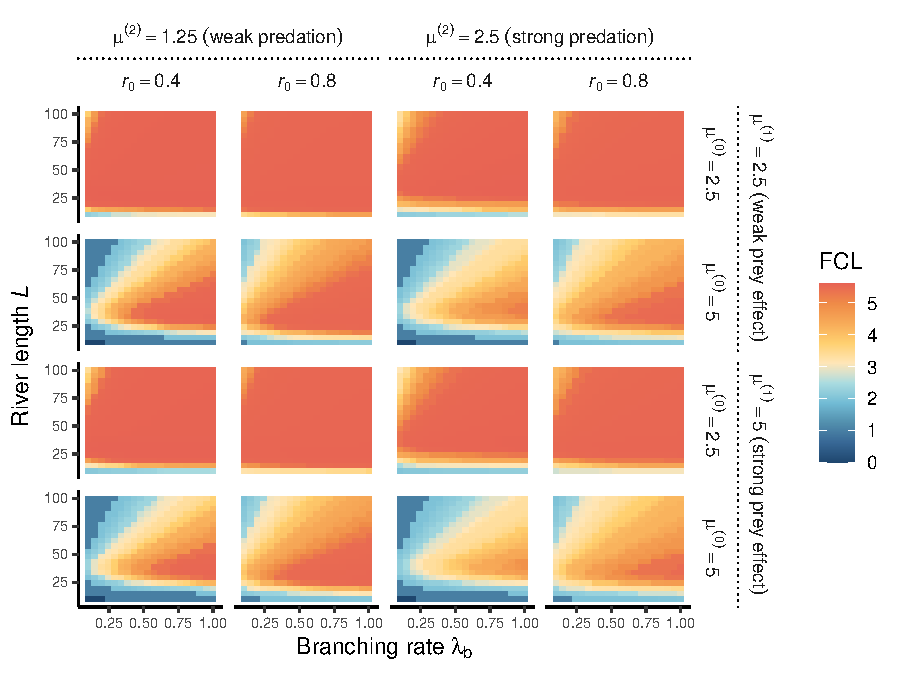
\includegraphics{../data_fmt/fig_rho025_g150_theta05.pdf}
\caption{Heatmap of FCL as a function of ecosystem size (river length,
\(L\)) and complexity (branching rate, \(\lambda_b\)), with rows and
columns displaying different combinations of resource supply (\(r_0\)),
disturbance regime (\(\mu^{(0)}\)), predation effect (\(\mu^{(c)}\)),
and prey effect (\(\mu^{(p)}\)). Each cell represents the average FCL of
five food webs. Additional parameter values are: number of gross
propagules \(g_0=150\), synchrony probability \(\rho=0.25\), omnivory
\(\theta=0.5\), habitat density \(h=2.5\), dispersal capability
\(\delta_0=0.5\), and scaling exponent \(\psi_1=\psi_2=0.5\).}
\end{figure}

\newpage

\subsection{Numerical prediction (low propagule, high synchrony, strong
omnivory)}\label{numerical-prediction-low-propagule-high-synchrony-strong-omnivory}

\begin{figure}
\centering
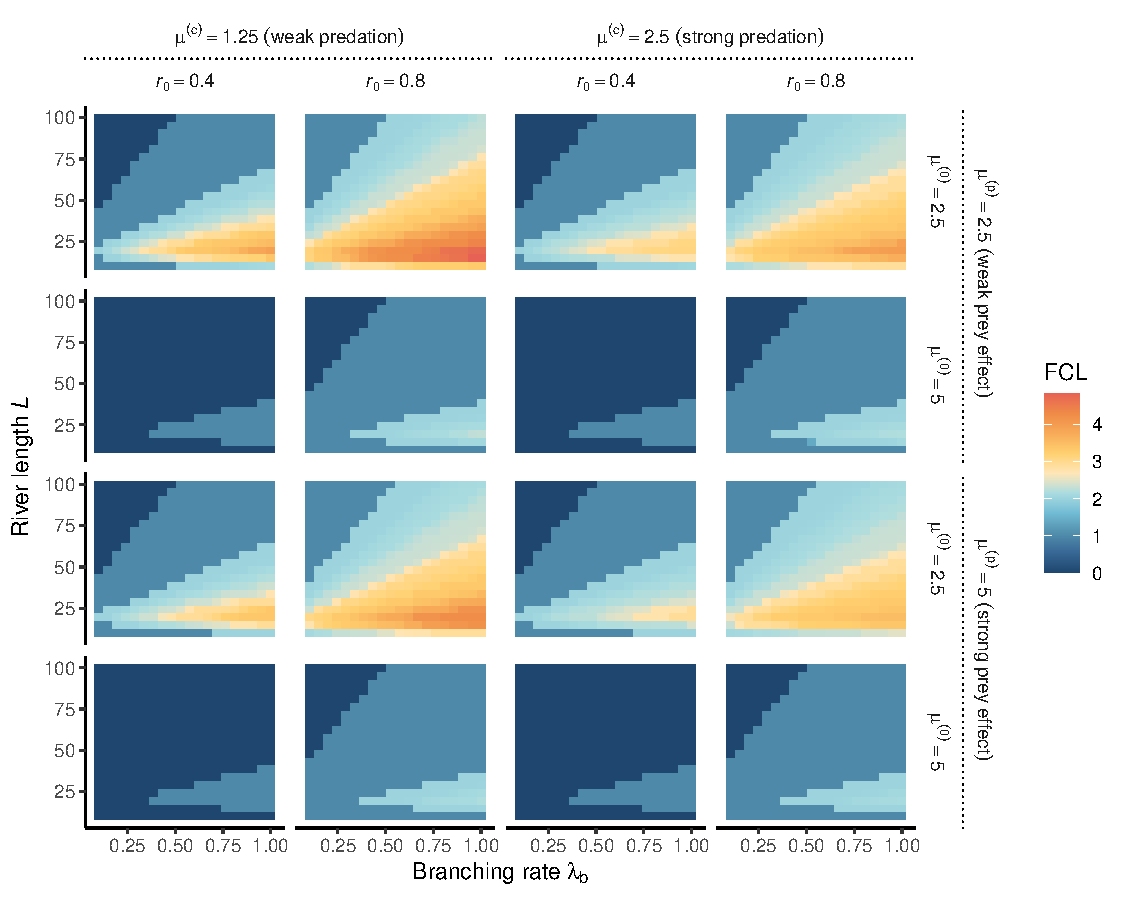
\includegraphics{../data_fmt/fig_rho05_g75_theta05.pdf}
\caption{Heatmap of FCL as a function of ecosystem size (river length,
\(L\)) and complexity (branching rate, \(\lambda_b\)), with rows and
columns displaying different combinations of resource supply (\(r_0\)),
disturbance regime (\(\mu^{(0)}\)), predation effect (\(\mu^{(c)}\)),
and prey effect (\(\mu^{(p)}\)). Each cell represents the average FCL of
five food webs. Additional parameter values are: number of gross
propagules \(g_0=75\), synchrony probability \(\rho=0.5\), omnivory
\(\theta=0.5\), habitat density \(h=2.5\), dispersal capability
\(\delta_0=0.5\), and scaling exponent \(\psi_1=\psi_2=0.5\).}
\end{figure}

\newpage

\subsection{Numerical prediction (high propagule, high synchrony, strong
omnivory)}\label{numerical-prediction-high-propagule-high-synchrony-strong-omnivory}

\begin{figure}
\centering
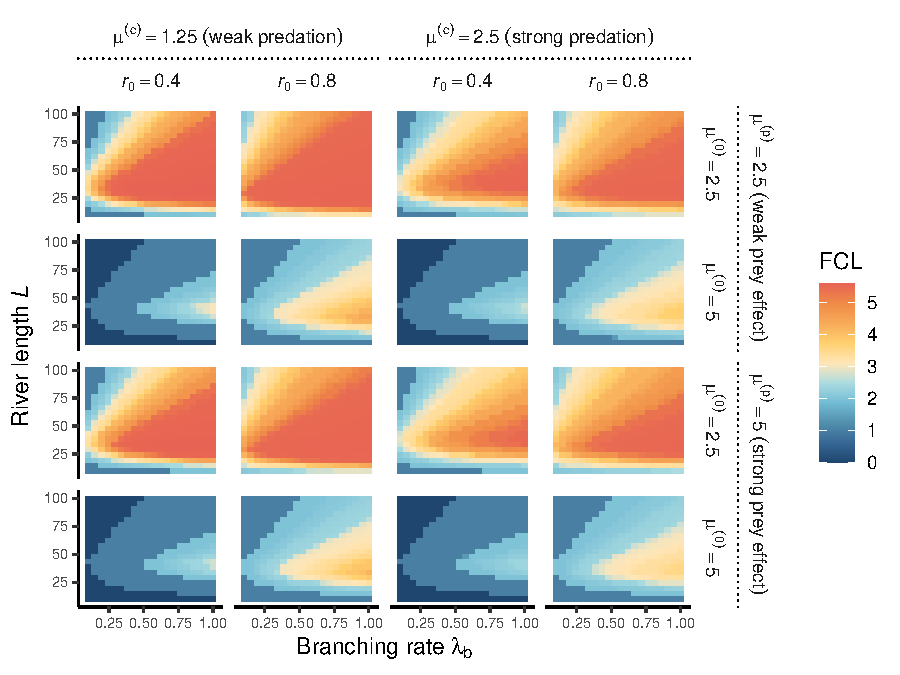
\includegraphics{../data_fmt/fig_rho05_g150_theta05.pdf}
\caption{Heatmap of FCL as a function of ecosystem size (river length,
\(L\)) and complexity (branching rate, \(\lambda_b\)), with rows and
columns displaying different combinations of resource supply (\(r_0\)),
disturbance regime (\(\mu^{(0)}\)), predation effect (\(\mu^{(c)}\)),
and prey effect (\(\mu^{(p)}\)). Each cell represents the average FCL of
five food webs. Additional parameter values are: number of gross
propagules \(g_0=150\), synchrony probability \(\rho=0.5\), omnivory
\(\theta=0.5\), habitat density \(h=2.5\), dispersal capability
\(\delta_0=0.5\), and scaling exponent \(\psi_1=\psi_2=0.5\).}
\end{figure}

\newpage
